\section{Introduction}


\subsection{Motivation}
  Concerns regarding the sustainability of using fossil fuels for energy generation
  have been raised as early as the 1970s \cite{rethinking_resource_depletion}. 
  One of the most well-known examples from that time was the 1972 report
  titled "Limits to Growth" by Meadows et. al. \cite{limits_to_growth}.
  In it a group of MIT scientists attempted to answer the question of
  how long will the Earth's natural resources last for
  considering the seemingly neverending growth of human civilisation.
  As a result of a conducted computer simulation,
  a rough estimate of around 100 years was given as a timeframe,
  after which the population would start to collapse due to a lack of resources.


  This estimate did not go without controversies back when it was first published.
  The methodology was thoroughly picked apart,
  leading many to dismiss the study findings
  \cite{rethinking_resource_depletion}.
  Naturally, nowadays, we are much better poised to verify
  the claims made by the now 50 year old book. The impeding resource depletion
  has certainly been made a less valid claim as technological progress
  made it possible to locate and tap into
  previously inaccesible fossil fuel fields
  \cite{shaping_the_global_oil_peak}.
  Taking into account other issues, however, 
  the original timeline of 100 years might have
  actually shifted closer. 


  When it comes to fossil fuel usage, in the last twenty years, 
  the primary concerns have changed from resource depletion to global warming 
  and irreversible environmental damage \cite{rethinking_resource_depletion}.
  In 2018 the Intergovermental Panel on Climate Change (IPCC) published a
  report indicating the need to stop the global temperature increase 
  at 1.5\degree C above the levels measurable in the pre-industrial era.
  Failure to do so is projected to lead to irreversible climate changes
  and in turn serious damage to human settlements around the world.
  \cite{ipcc2018}


  Fossil fuels account for as much as 70\% of greenhouse gas emissions.
  Electricity generation alone causes 25-35\% 
  \cite{global_climate_change} of the total amount.
  Such a high share means that reducing this output
  is going to be crucial in meeting the goals outlined by the IPCC.
  At the beginning of the twentieth century, renewable energies, i.e. 
  wind, solar, biomass and geothermal were thought
  to be the perfect solution to the issue at hand
  \cite{renewable_review_2000}. 


  In modern times, we have now become aware of multiple issues
  that make renewable energy generation a problem at large scale.
  Most importantly, their efficacy varies depending on the geographical
  location and climate. Even when placed in optimal conditions,
  they do not offer perfect stability. Additionally, the land
  usage is greater than the traditional forms of energy production
  \cite{renewable_problems}.

\subsection{Fission energy}

  The drawbacks of renewable energies have led to a formation
  of an alternative approach in both research and policymaking. 
  The use of nuclear energy for supplementing the shortcomings 
  of renewables has been suggested as a potential path forward.
  This concept is referred to as hybrid nuclear-renewable system.
  \cite{hybrid_nuclear_renewable}. 

  There are two ways that nuclear energy can be created and harnessed.
  In the more well-established technology, fission, heavy atoms 
  (usually Uranium) are bombarded with neutrons 
  and split into two or more lighter nuclei and
  additional neutrons as shown in \autoref{fig:fission}.
  The reaction is self-sustaining 
  and releases energy in the form of heat that is then used
  to boil water. The steam causes turbines to spin
  and generate electricity.
	\begin{figure}[h]
	  \centering
	  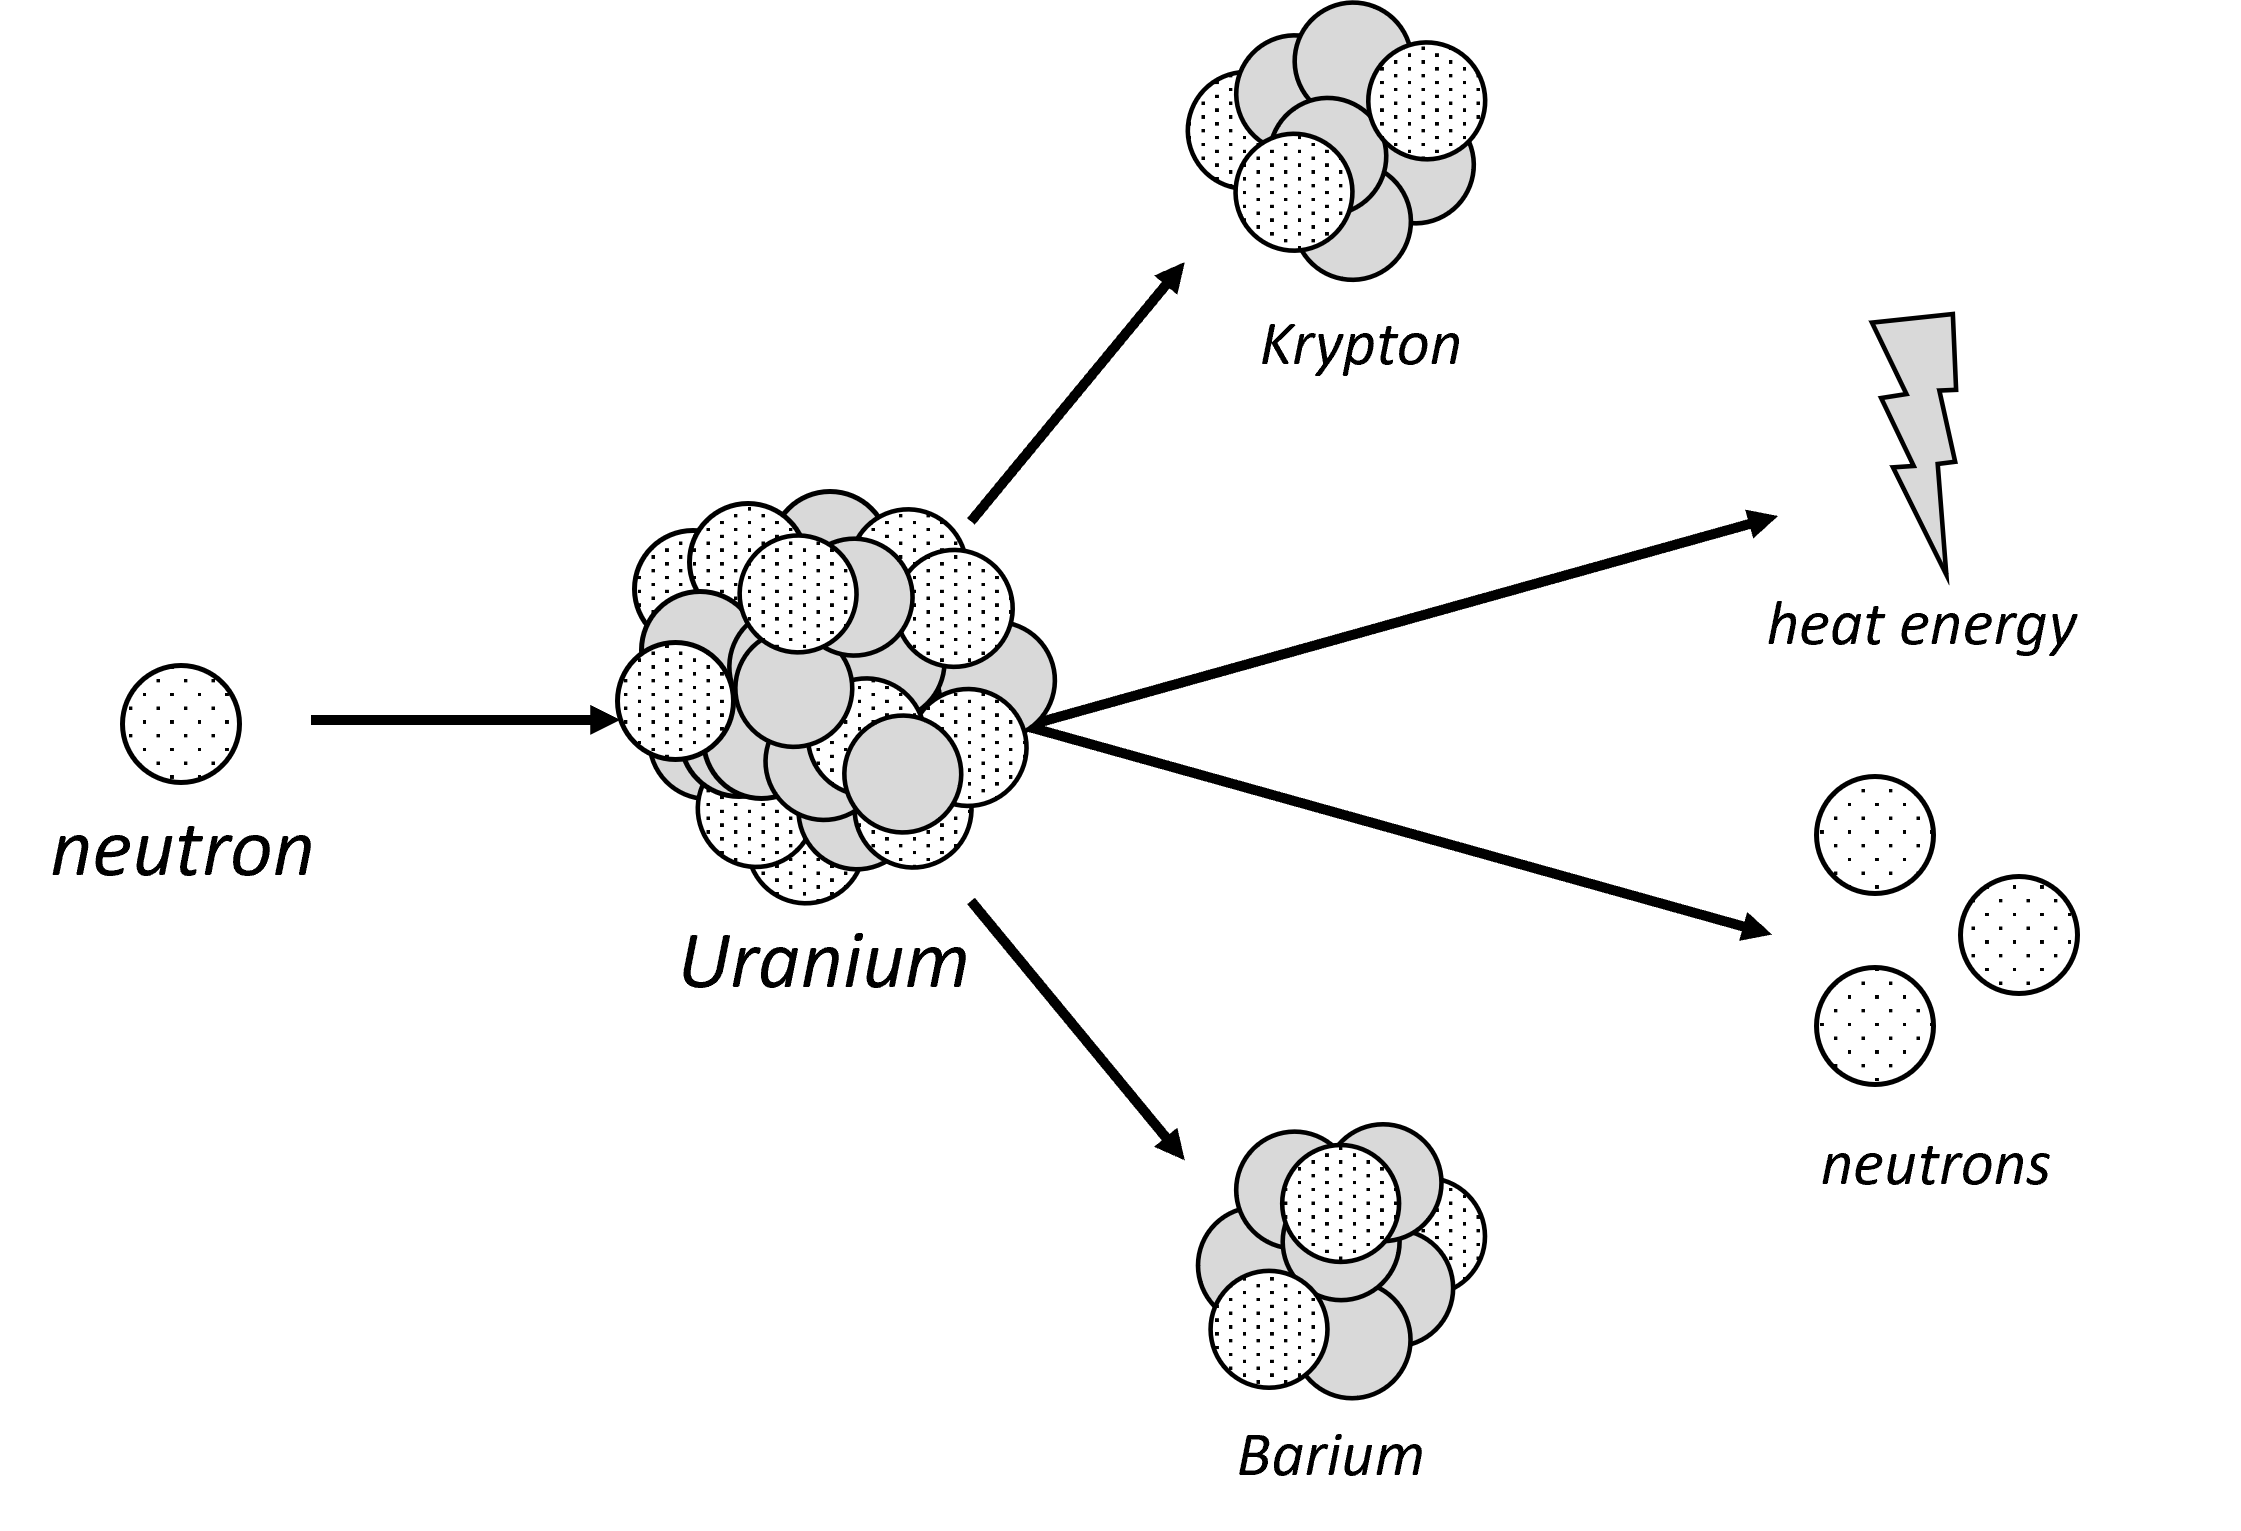
\includegraphics[width=.85\linewidth]{media/fission.png}
	  \caption{Uranium fission reaction}
	  \label{fig:fission}
	\end{figure}

  Fission is far from a new concept, as first fission reactors have been 
  built as early as 1942 \cite{first_fission_reactor}. 
  Although the technology itself is quite old 
  and has been greatly improved over time, 
  there is reasonable reluctance to build and use fission power plants. 
  The issue that gets raised most often is the storage of radioactive waste. 
  There are, however, multiple less well-known
  problems with fission \cite{fission_problems}. 


  The tragedies of Chornobyl and Fukushima reactors
  have caused many people to be wary of fission. However, even if
  democratic support is disregarded in policymaking, the acquisition,
  storage and disposal of radioactive materials required for and produced 
  during fission prove to be an administrative challenge, especially 
  if reactor construction and maintenance is to be handled
  by private entities \cite{fission_tech_and_current_issues}. 
  The complexity of the problem suggests that 
  as we arrive to more concrete solutions we 
  should not stop exploring other potential alternatives.

\subsection{Fusion energy}

  Just like it is possible to split atoms, it is also possible to
  combine them together in a process referred to as fusion. 
  Fusing atoms lighter than Iron is a reaction that 
  can produce surplus energy as highlighted by \autoref{fig:binding_energy}.
  Two atoms of low binding energy can fuse into an atom of higher 
  binding energy, releasing heat based on the mass-energy equivalence formula.
  The output energy can be used to generate electricity in
  the exact same manner as with fission. 
  The problem with fusion reactors is that the conditions necessary
  for fusion to happen are extremely harder to achieve and sustain 
  \cite{structural_materials_fusion}.
	\begin{figure}[h]
	  \centering
	  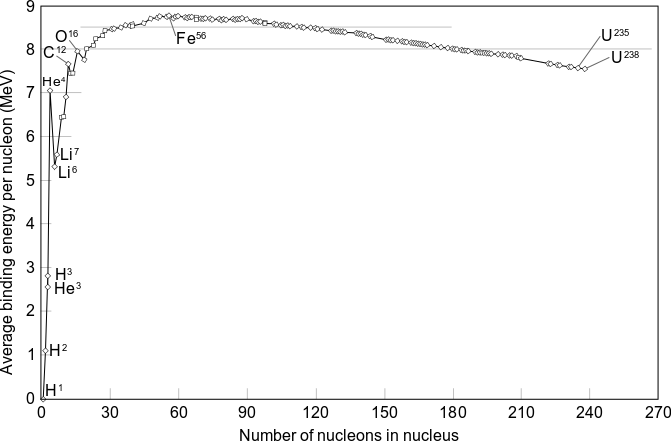
\includegraphics[width=.85\linewidth]{media/binding_energy.png}
	  \caption{Average binding energy per nucleon as a function of the number of nucleons in the atom}
	  \label{fig:binding_energy}
	\end{figure}

  Fusion is the primary reaction that causes stars to emit light and heat.
  The reaction that is most often artificially attempted on Earth differs
  from that occurring naturally in the Sun. There, a p-p reaction occurs. 
  This means the need of converting 4 protons into ${}^{4}$He.
  Replicating this reaction on a larger scale is extremely challenging 
  due to the need to convert protons into neutrons.
  On Earth, fusion experiments primarily rely on using hydrogen isotopes, 
  most commonly deuterium (D) and tritium (T) shown in \autoref{fig:fusion}.
	\begin{figure}[h]
	  \centering
	  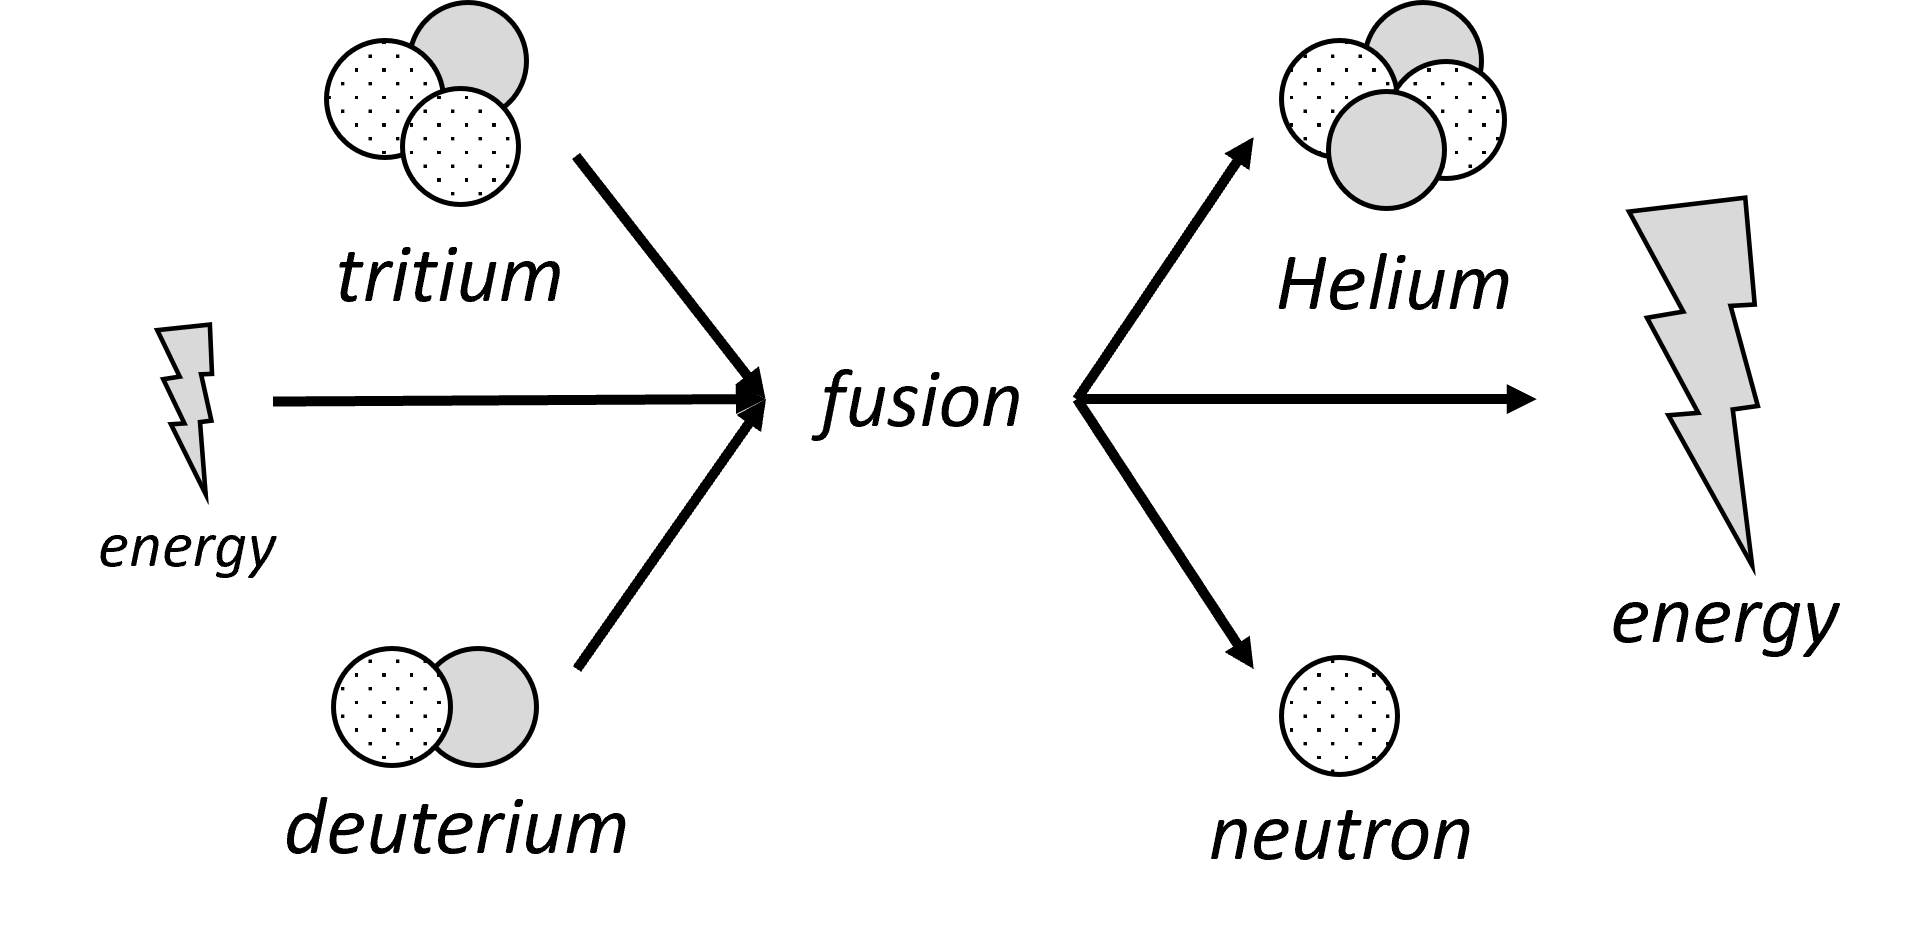
\includegraphics[width=.75\linewidth]{media/fusion.png}
	  \caption{D-T fusion reaction}
	  \label{fig:fusion}
	\end{figure}



  Despite being an easier approach, it still requires us to sustain
  a 200 million \degree C plasma. This means that an enormous amount of energy
  must be used to first heat the plasma up and then confine it to 
  prevent it from completely destroying the reactor. 
  The efficiency of D-T reactions might, however, worth the trouble.
  Theoretically, just 30 mg of deuterium would generate as much energy
  as 250 l of gasoline \cite{nuclear_fusion_status}. 


  Such numbers sound incredible, but there are naturally multiple drawbacks too.
  Tritium, the other input material of this most promising reaction is
  extremely rare in nature. Its artificial production is currently 
  done only by a select number of facilities. 
  Combined with its relatively short half-life of around 12 years, 
  there are fears of it running out. It is proven that fusion reactors
  will be capable of "breeding" their own tritium, however the transition period 
  may still prove to be troublesome \cite{fusion_fuel_running_out}.


  In the end, despite being a similarly old technology as fission
  \cite{fusion_history},
  a fusion reactor with a net positive energy balance
  has not yet been constructed. Containing plasma heated to such extreme
  temperatures cannot be achieved with any solid material and must 
  be done with the use of inertial or magnetic forces. 
  The most common reactors that employ this concept are:
  tokamaks (\autoref{fig:iter_reactor}) 
  and stellarators (\autoref{fig:w7x_reactor}).
  The former design has been selected for probably
  the most ambitious fusion project to date, 
  the International Thermonuclear Experimental Reactor (ITER)
  \cite{nuclear_fusion_status}.

  \begin{figure}[h]
    \centering
    \begin{minipage}{.5\textwidth}
      \centering
      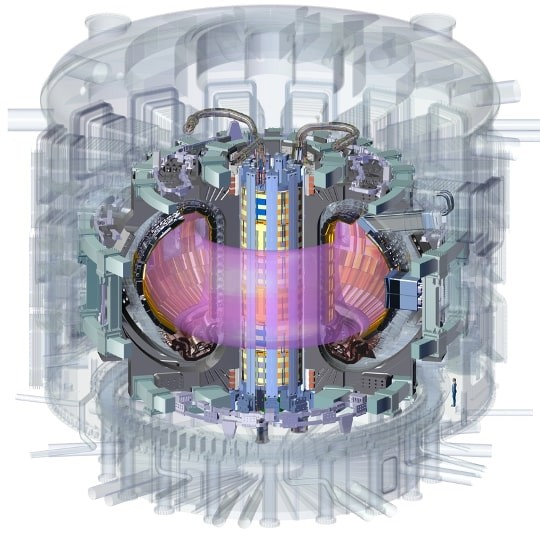
\includegraphics[width=.5\linewidth]{media/iter_reactor_3d.jpeg}
      \caption{ITER tokamak model\cite{iter_website}}
      \label{fig:iter_reactor}
    \end{minipage}%
    \begin{minipage}{.5\textwidth}
      \centering
	  \includegraphics[width=.65\linewidth]{media/w7x_3d.png}
      \caption{Wendelstein W7X sterellator model\cite{w7x_website}}
      \label{fig:w7x_reactor}
    \end{minipage}
  \end{figure}

\subsection{ITER Tokamak Project}
  \subsubsection{Tokamak}
	\begin{figure}
	  \centering
	  \includegraphics[width=.75\linewidth]{media/iter_crosssection.jpeg}
	  \caption{ITER tokamak cross section\cite{iter_website}}
	  \label{fig:iter_crosssection}
	\end{figure}
	Tokamaks are reactors composed of a toroidal vacuum chamber surrounded by
	massive electromagnetic coils as shown in \autoref{fig:iter_crosssection}.
	The magnetic fields are used to shape plasma 
	and keep it away from the device internal walls. 
	Operation starts with the removal of air and impurities from the vessel.
	The gaseous fuel is introduced and a strong current is induced 
	ionizing the gases, thus forming plasma. Additional heat is introduced with
	microwave and fuel injections. Particles within the
	formed plasma can then collide with such force that they begin
	to break through atomic repulsion and fuse producing a large amount of energy.
	\cite{iter_website}
  \subsubsection{ITER Goals}

	At 24 m height and 30 m width, 
	ITER will be the biggest tokamak ever constructed. 
	That's twice as big as the largest experimental reactor currently in service, 
	the Joint European Torus (JET). JET has been working since 1983 with 
	a goal of achieving net energy gain. Despite running successful 
	plasma experiments and recently starting deuterium-tritium experiments,
	the highest fusion energy gain Q 
	(the ratio of produced power to the power required to sustain the plasma)
	obtained by JET was 0.33. A record only recently topped by a different 
	type of a fusion device held at the US Department of Energy’s
	National Ignition Facility. Using laser technology it was possible to
	obtain a Q of 0.7 for 4 billionths of a second. \cite{fusion_records}
	

	Although not supposed to work as a power plant, just an experiment,
	throughout its operation ITER intends to break this record by a lot.
	The new reactor is designed to reach an energy gain of 10 
	for the duration of a few minutes. This is of course still a theoretical
	plan, as the facility is still a fairly long time from being finished.
	As of 2022, the vacuum vessel is yet to be welded together\cite{iter_timeline}.
	First plasma operation is scheduled for the end of 2025\cite{iter_timeline},
	although multiple delays have already happened in the past \cite{iter_delays},
	so future ones would at this point not be too surprising. 
  \autoref{fig:iter_aerial} shows an aerial picture of ITER from 14th of April 2020.
  Not all facilities have been fully constructed at this time.
	\begin{figure}[h]
	  \centering
	  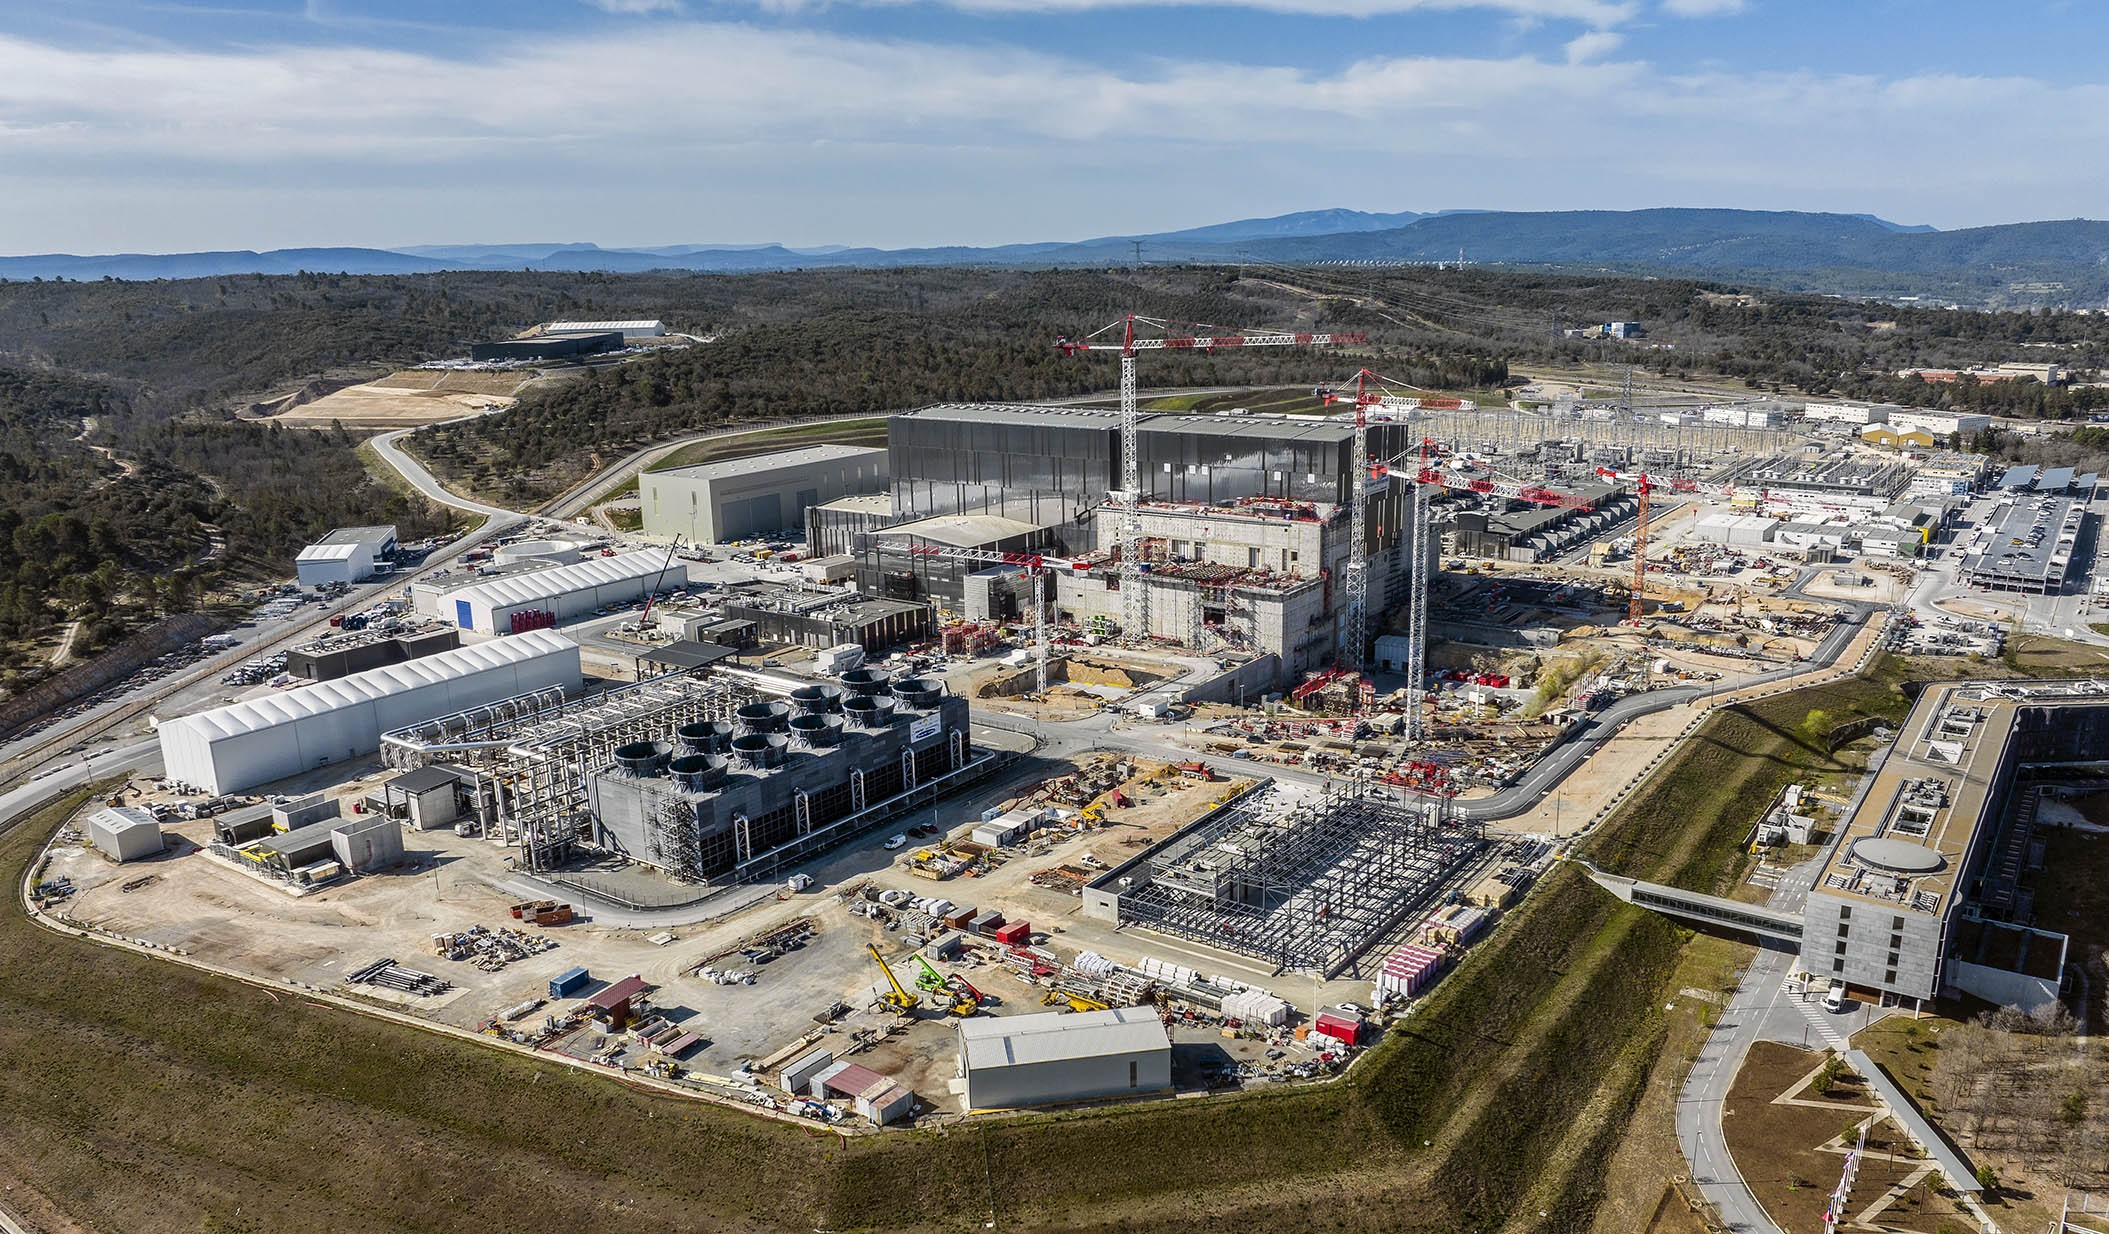
\includegraphics[width=.9\linewidth]{media/iter_aerial_2022.jpg}
	  \caption{Aerial view of the ITER facility as of 2022\cite{iter_website}}
	  \label{fig:iter_aerial}
	\end{figure}
	\subsubsection{Primary Concerns}

	With a project of this magnitude it is near impossible to predict
	everything that might go wrong. There are naturally safety concerns,
	questions regarding the ambitious goals set by the management and
	the troubles of international cooperation\cite{iter_delays}.
	It is thus crucial to maintain maximum operational safety 
	and log all experimental data. This should ensure that even in the 
	case of partial failure of the project important practical knowledge
	can be recorded for future fusion experiments.


	When operational, ITER will rely on around 50 completely different
	measurement systems to control, evaluate and investigate its plasma 
	\cite{iter_diagnostics_count}.
	This translates into dozens of gigabytes of data being generated, 
	processed and archived every second as the experiment is running 
	\cite{iter_data_throughput}.
	With some of the experiments lasting fractions of a second,
	a lot of the critical data acquisition and control must occur
	in real time and without waiting for human reaction 
	\cite{iter_realtime_processing}.
	This poses an important challenge when it comes to the choice
	of computing apparatus. A perfect device would offer
	infinite configurability preferably with remote access 
	as well as a very high data throughput. 

	Traditional computers or more precisely Central Processing Units (CPUs) 
	are remotely reprogrammable but may offer insufficient speeds in 
	some of the real time applications. On the other end of this scale lie 
	Application Specific Integrated Circuits (ASIC). These devices are an 
	arrangement of digital logic gates realizing one specific goal, like 
	digital signal filtering or processing network packets.
	ASICs offer unmatched bandwidth but cannot really be reconfigured
	after deployment, making them a risky choice in highly experimental
	applications such as tokamaks.

\subsection{Field Programmable Gate Arrays}
Devices that offer a compromise between speed and reconfigurability
exist nowadays. Most commonly Field Programmable Gate Arrays (FPGAs) are used.
FPGAs are formed out of matrices of so called Configurable Logic Blocks (CLBs).
These are small circuits that produce a single bit of logic output
out of 4 input bits, using a reprogrammable function. These blocks 
are then wired together using programmable interconnects. Such design 
allows for the implementation of very efficient digital algorithms
directly with the use of logical gates, without the need for an
entire processor. \cite{xilinx_what_is_fpga}


The interconnects and CLB internal structure introduce additional wiring
that would be unnecessary in the case of ASICs. These stray capacitances 
and inductances limit the maximum clock speed of FPGAs. This not too much
of an issue provided that the function can be parallelised. To offset 
this limitation, most FPGAs manufactured today come packed with 
more complex sub-circuitry that can be intermixed with the CLBs
as indicated in \autoref{fig:fpga_structure}.
These components can vary greatly from fast arithmetical blocks
to small CPU-based microcontrollers.

	\begin{figure}[h]
	  \centering
	  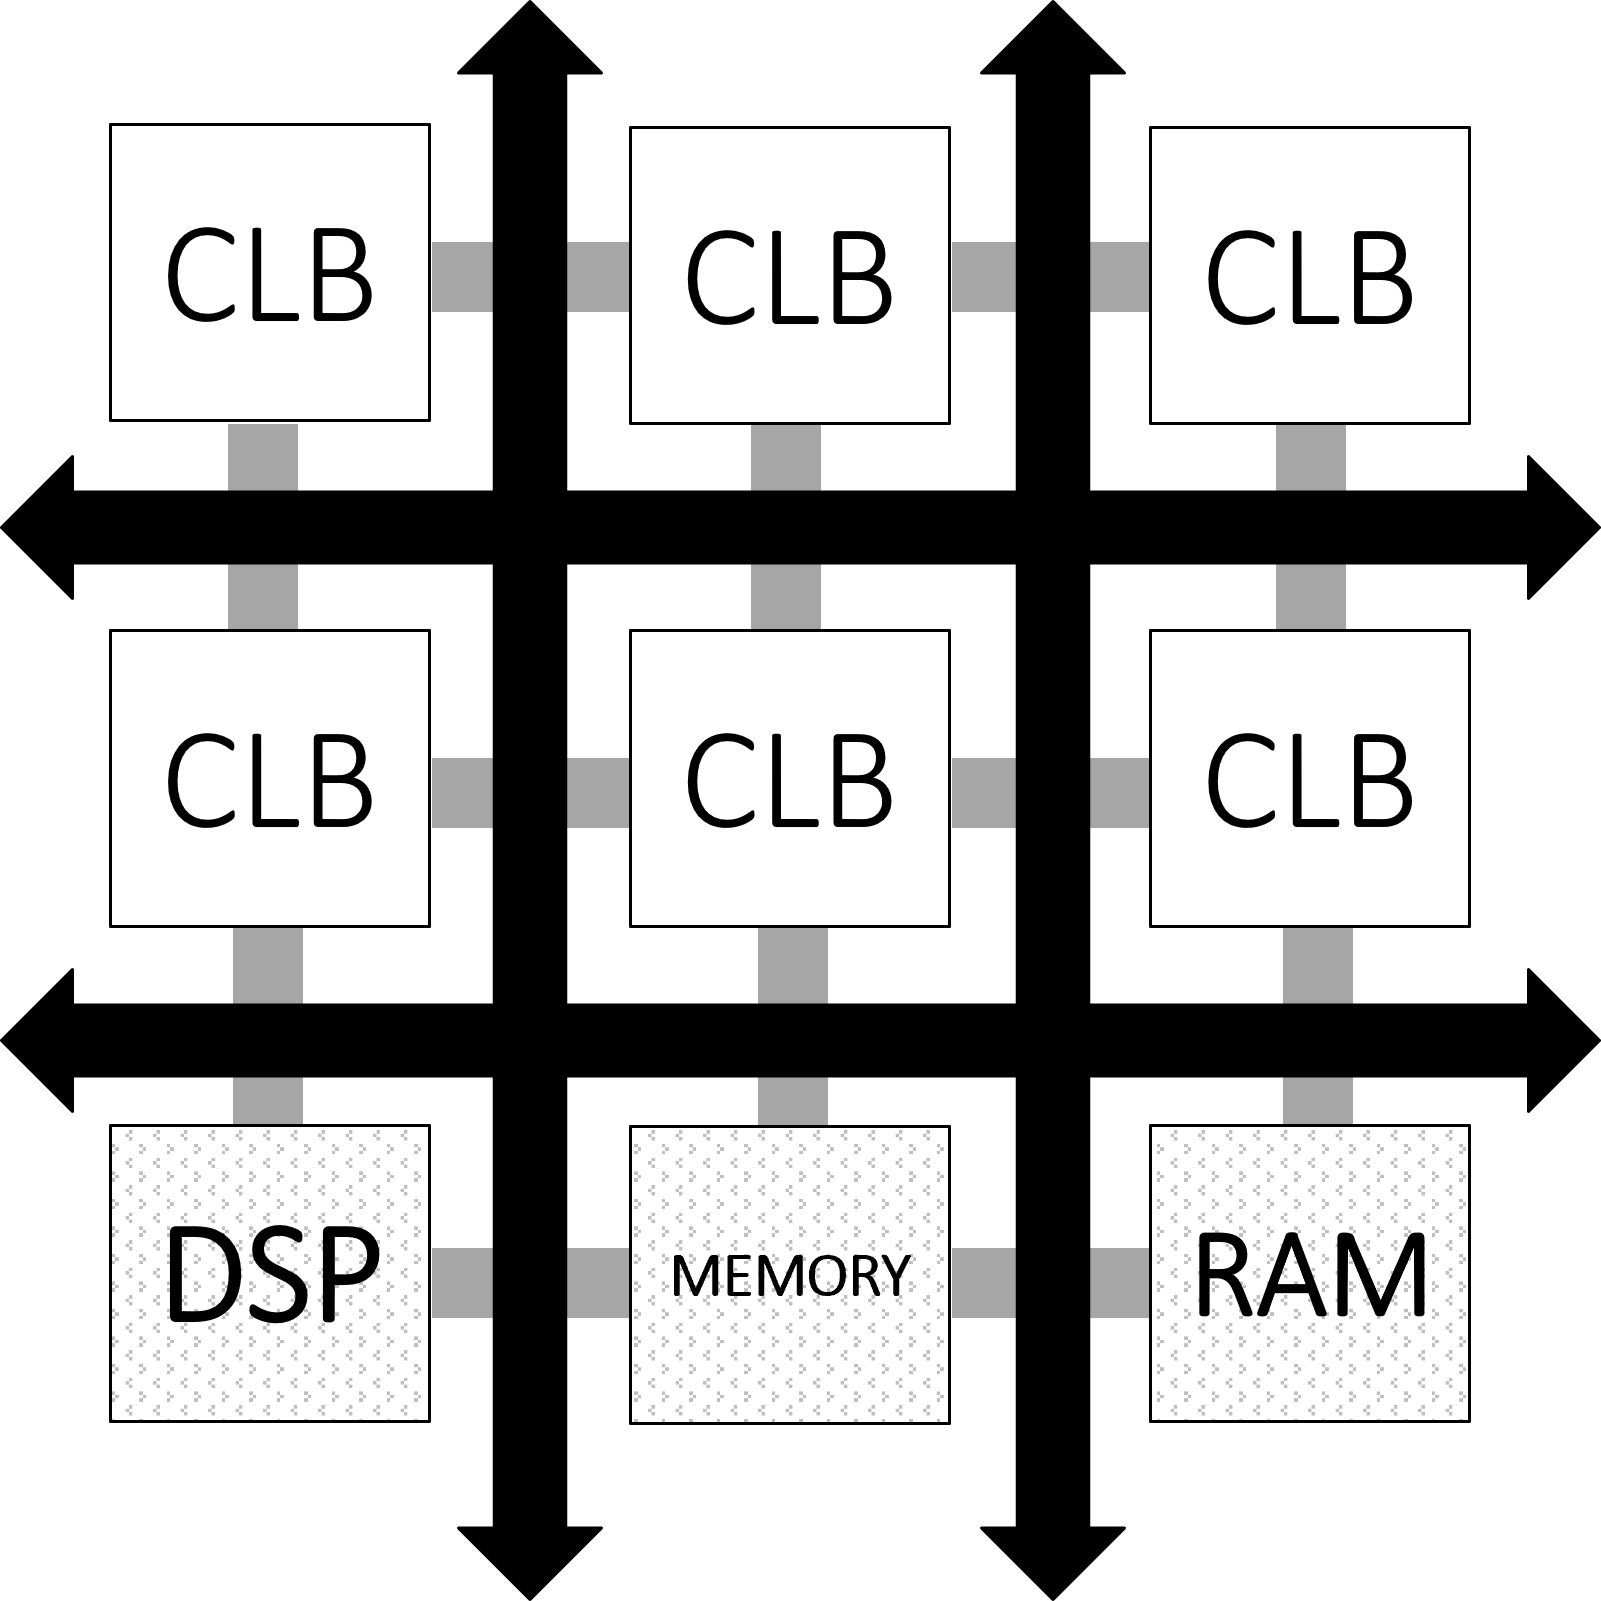
\includegraphics[width=.6\linewidth]{media/fpga_structure.png}
	  \caption{The internal structure of an FPGA}
	  \label{fig:fpga_structure}
	\end{figure}
\subsection{Problem statement}

The nature of FPGAs makes them instrumental in the data acquisition 
and control systems of modern fusion experiments like the ITER tokamak.
This work evaluates the potential usage of Field Programmable Gate Arrays
for the detection and analysis of pulses produced by PhotoMultiplier Tubes (PMTs)
being part of a High X-Ray Monitor (HXRM) designed to monitor Runaway Electorns
(REs) at tokamaks.


A functional system for the Digital Pulse Processing (DPP) at the rate of 
1 GS/s is proposed and implemented in an FPGA. A custom
software package for control and data acquisition is shown.
The optimization of both hardware and software is described.
Different algorithms for pulse detection and discrimination
are analysed, simulated and implemented in hardware. Finally design
considerations for future systems are given.

